\section{Ambiente de Referênciamento Local} 
\label{sec:ambiente_de_referenciamento_local}
Variáveis que são definidas dentro de subprogramas são chamadas de variáveis locais, porque o acesso a elas normalmente é restrito ao subprograma na qual são definidas \cite{sebesta}. Essas variáveis podem ser variáveis estáticas ou variáveis dinâmicas na pilha.

\subsection{Variáveis Locais}
\label{sub:variaveis_locais}
Variáveis estáticas são vinculadas a células de memória antes do inicio da execução do programa e continuam até o término de sua execução.Uma das vantagens de variáveis estáticas é que elas possuem um endereçamento direto na memória como mostra a figura \ref{enderecamento}, permitindo assim um acesso mais rápido em relação a variáveis com endereçamento indireto. Outra vantagem, é por não causarem sobrecarga em tempo de execução para alocação de desalocação. Uma desvantagem das variáveis estáticas é por não se comportarem bem em subprogramas recursivos. Considere a listagem \ref{lst:recursivo_c} de uma função em C, onde a saída após a execução do programa será 6, 12 e 18.

\begin{lstlisting}[caption={Programa recursivo com variável estática}, label={lst:recursivo_c}]
#include <stdio.h>

int sum ( int arr[], int n )
{
    static int result = 0;
    if (n == 0)
        return result ;
    else {
        result += arr[n - 1];
        sum(arr, n - 1);
     }
}

int main(void) {
    int array[5] = {1,2,3,4,5};
    printf("%d\n", sum(array, 3));
    printf("%d\n", sum(array, 3));
    printf("%d\n", sum(array, 3));
    return 0;
}
\end{lstlisting}

Variáveis dinâmicas na pilha, são vinculadas ao armazenamento quando o subprograma inicia sua execução e desvinculadas do armazenamento quando ele se encerra. Variáveis desse tipo permitem maior flexibilidade para subprogramas (por exemplo, subprogramas recursivos), além de permitir o compartilhamento de parte do armazenamento para variáveis locais de todos subprogramas (não ativos ao mesmo tempo). Porém, variáveis dinâmicas na pilha possuem algumas desvantagens como o enderaçamento indireto \ref{enderecamento} e o tempo gasto para inicialização (se necessário), alocação e desalocação. 

Linguagens como ALGOL 60 e suas linguagens descendentes, possuem variáveis locais dinâmicas na pilha. Em funções em C as variáveis são dinâmicas na pilha a menos que sejam especificamente declaradas como \textbf{static}. Subprogramas Pascal e Ada e métodos em C++, Java, C\# têm somente variaveis dinâmicas na pilha. 

\begin{figure}[ht!]
 \centering
 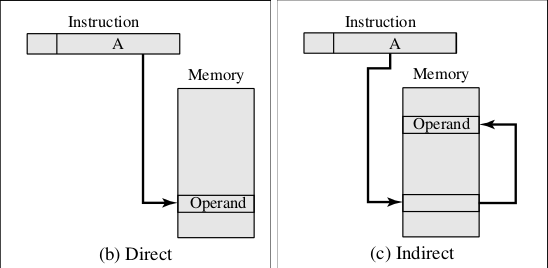
\includegraphics[scale=0.65]{./imagens/enderecamento.png}
 \caption{Endereçamento direto e indireto \cite{stallings}}
\label{enderecamento}
\end{figure}

\subsection{Aninhamento de Subprogramas} 
\label{sub:aninhamento_de_subprogramas}
Linguagens como ALGOL 68, Pascal e Ada permitem aninhamento de subprogramas, assim como linguagens mais recentes como JavaScript, Python e Lua. Linguagens descententes de C não permitem aninhamento. O trecho de código a seguir mostra um exemplo de aninhamento de funções em JavaScript.

\begin{verbatim}
function hipotenusa(a, b) {
   function quadrado(x) {
      return x * x; 
   }
   return Math.sqrt(quadrado(a) + quadrado(b));
}
\end{verbatim}